\begin{landscape}
	\begin{figure}[H]
		\centering
		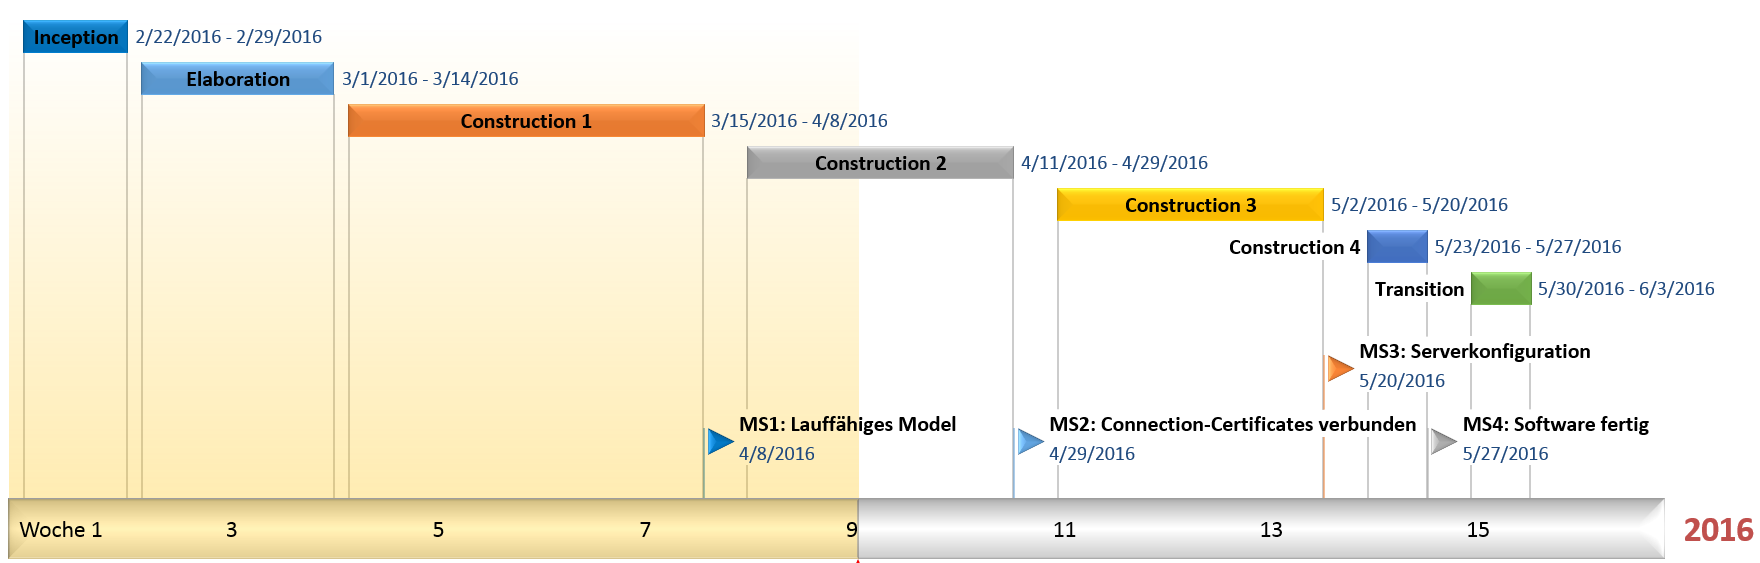
\includegraphics[width=250mm]{images/gantt.PNG}
		\caption{Gantt Chart}
	\end{figure}
\section{Risiken}
Um den Problemen, die während des Projekts auftreten können entgegenzuwirken, haben wir eine Risiko Analyse durchgeführt. Diese konnte dann bei der Planung eingesetzt werden.

\subsection{Technische Risiken}
\begin{table}[H]
    \begin{tabular}{|p{0.4cm}|p{2.5cm}|p{7cm}|p{1.5cm}|p{2.25cm}|p{1.75cm}|p{3cm}|p{4cm}|}
    \hline    
    \rowcolor{lightblue}
    Nr & Titel & Beschreibung & maximaler Schaden & Eintrittswahr-scheinlichkeit & Gewichteter Schaden & Vorbeugung & Verhalten beim Eintreten \\ \hline
	R1 & Python Crypto Library & Die evaluierte Crypto Library für die Zertifikaterkennung ist fehlerhaft oder ungenügend. & 50h & 20\% & 10h & Evaluation Library & Zertifikate werden nicht mehr ausgelesen, sondern nur noch stupid importiert. \\ \hline
	R2 & Komplexität VICI-Schnittstelle & Die Python Vici Schnittstelle deckt sich nicht mit der swanControl Notation. Dadurch kann massiv mehr Aufwand während der Implemenation entstehen. & 50h & 40\% & 20h & Die Vici Schnittstelle muss mit dem Prototypen gut durchgetestet werden, um Fehler möglichst früh zu finden. & Kontakt mit Tobias Brunner aufnehmen \\ \hline
	R3 & Einrichten automatisierte Testumgebung & Aufbau und Einrichten einer Integrationtestumgebung, welche es erlaubt Ipsec Tunnels zwischen mehreren Rechnern aufzubauen. & 60h & 60\% & 36h & Informationen zu CI Anbieter sammeln & Eigene Infrastruktur verwenden. \\ \hline
    \end{tabular}
    \caption[Risiken]{Risiken - Die technischen Risiken wurden zu Beginn des Projektes, wie in der Tabelle ersichtlich, definiert.}
\end{table}
\end{landscape}

\subsection{Auswertung}
\paragraph{R1 Python Crypto Library} Mit Hilfe der Evaluation der Crypto Library konnte dieses Risiko aus dem Weg geräumt werden. Der Aufwand blieb im erwarteten Rahmen und mit \textbf{oscrypto} wurde eine passende pure Python Bibliothek gefunden werden.

\paragraph{R2 Komplexität VICI-Schnittstelle} Das Zusammenspiel zwischen Pyhton/Django funktionierte nahtlos und wie in der Dokumentation beschrieben. Problematischer und Zeitintensiver war jedoch das korrekte Konfigurieren von strongSwan. Die 

\paragraph{R3 Einrichten automatisierte Testumgebung}
Docker-compose legte die Grundsteine, welche es uns ermöglichten mehrere Rechner für die Testumgebung zu nutzen. Da der uns wohl bekannte CI Anbieter Travis dies zudem noch unterstützt wurden automatische Integrationtest möglich. Das Finden einer passenden Lösung war ohne grössere Komplikationen möglich. Mehr Aufwand als erwartet, gab jedoch die Konfiguration der Docker-Container. Womit dieses Risiko teils eintrat.\\
\medskip
\begin{table}[H]
	\centering
    \begin{tabular}{|p{2cm}|l|p{2cm}|}
    \hline    
    \rowcolor{lightblue}
	Nr & Titel & Schaden \\ \hline   
	R1 & Python Crypto Library & 0h \\ \hline
	R2 & Komplexität VICI-Schnittstelle & 0h \\ \hline
	R3 & Einrichten automatisierte Testumgebung& 0h \\ \hline
	\rowcolor{lightblue}
	Total &  & 0h \\ \hline
    \end{tabular}
    \caption[Risikoauswertung]{Risikoauswertung}
\end{table}